\documentclass{diploma}

\student{Ефименко Кирилл Игоревич}
\group{М8О-409Б-22}
\theme{Система индексации ончейн-данных}

\supervisor{Филимонов Николай Сергеевич}
\firstConsultant{Булакина Мария Борисовна}
\reviewer{Филимонов Николай Сергеевич}

\faculty{№ 8 <<Компьютерные науки и прикладная математика>>}
\department{806}
\speciality{01.03.02 <<Прикладная математика и информатика>>}
\profile{Информатика}

\departmentFullName{№ 806}
\headOfDepartment{Крылов Сергей Сергеевич}

% Дата. Оставляем пустое место для дня
\date{\uline{\hspace{24pt}} мая \the\year\ года}

\newacronym{api}{API}{Application Programming Interface}
\newacronym{c4}{C4}{Context, Containers, Components, Code}
\newacronym{cli}{CLI}{Command Line Interface}
\newacronym{db}{БД}{база данных}
\newacronym{dfd}{DFD}{Data Flow Diagram}
\newacronym{etl}{ETL}{Extract, Transform, Load}
\newacronym{http}{HTTP}{HyperText Transfer Protocol}
\newacronym{https}{HTTPS}{HyperText Transfer Protocol Secure}
\newacronym{json}{JSON}{JavaScript Object Notation}
\newacronym{jsonrpc}{JSON-RPC}{протокол удаленного вызова процедур поверх JSON}
\newacronym{mtls}{mTLS}{mutual TLS}
\newacronym{mvp}{MVP}{Minimum Viable Product}
\newacronym{openapi}{OpenAPI}{OpenAPI Specification}
\newacronym{fk}{FK}{Foreign Key}
\newacronym{pk}{PK}{Primary Key}
\newacronym{rest}{REST}{Representational State Transfer}
\newacronym{rpc}{RPC}{Remote Procedure Call}
\newacronym{sql}{SQL}{Structured Query Language}
\newacronym{tls}{TLS}{Transport Layer Security}
\newacronym{ui}{UI}{User Interface}
\newacronym{utxo}{UTXO}{Unspent Transaction Output}
\newacronym{yaml}{YAML}{YAML Ain't Markup Language}

\newglossaryentry{term-onchain-data}{
    name={Ончейн-данные},
    description={данные, зафиксированные в блокчейне, а также производные представления, формируемые на их основе для прикладного анализа}
}
\newglossaryentry{term-indexer}{
    name={Индексер},
    description={серверное приложение, которое получает данные блокчейна, нормализует их, сохраняет в базе данных и предоставляет прикладной API}
}
\newglossaryentry{term-bitcoin-core}{
    name={Bitcoin Core},
    description={программная реализация узла сети Bitcoin, используемая как доверенный источник первичных блоков и транзакций}
}
\newglossaryentry{term-bitcoin}{
    name={Bitcoin},
    description={децентрализованная блокчейн-сеть и одноименная криптовалютная система, данные которой являются предметом индексации}
}
\newglossaryentry{term-canonical}{
    name={Каноническая цепь},
    description={актуальная ветвь блокчейна Bitcoin, признаваемая основной в рассматриваемый момент времени}
}
\newglossaryentry{term-job}{
    name={Задание индексирования},
    description={управляемый процесс обработки блокчейн-данных с собственным идентификатором, статусом, прогрессом и параметрами выполнения}
}
\newglossaryentry{term-reorg}{
    name={Reorg},
    description={смена канонической ветви блокчейна, из-за которой ранее принятые блоки и транзакции становятся неканоническими}
}
\newglossaryentry{term-mempool}{
    name={Mempool},
    description={множество неподтвержденных транзакций, известных узлу Bitcoin Core и ожидающих включения в блок}
}
\newglossaryentry{term-stateless}{
    name={Stateless-сервис},
    description={сервис, который не хранит критичное состояние локально между перезапусками и размещает его во внешнем хранилище}
}
\newglossaryentry{term-address-index}{
    name={Адресный индекс},
    description={структура данных, позволяющая быстро находить транзакции, выходы, балансы и mempool-события, связанные с конкретным адресом}
}
\newglossaryentry{term-address-balance}{
    name={Адресный баланс},
    description={агрегированное значение суммы непотраченных выходов или исторического состояния адреса на определенный момент цепи}
}
\newglossaryentry{term-utxo}{
    name={UTXO},
    description={непотраченный выход транзакции, который может быть использован как вход последующей транзакции}
}
\newglossaryentry{term-postgresql}{
    name={PostgreSQL},
    description={реляционная система управления базами данных, используемая для хранения блоков, транзакций, UTXO, балансов, заданий и метрик состояния}
}
\newglossaryentry{term-rust}{
    name={Rust},
    description={язык программирования, на котором реализована серверная часть системы}
}
\newglossaryentry{term-python}{
    name={Python},
    description={язык программирования, используемый для реализации командного интерфейса проекта}
}
\newglossaryentry{term-react}{
    name={React},
    description={JavaScript-библиотека, используемая при реализации административной панели}
}
\newglossaryentry{term-vite}{
    name={Vite},
    description={инструмент сборки frontend-приложений, применяемый для административной панели}
}
\newglossaryentry{term-docker}{
    name={Docker},
    description={платформа контейнеризации, применяемая для воспроизводимой сборки и развертывания компонентов системы}
}
\newglossaryentry{term-docker-compose}{
    name={Docker Compose},
    description={средство описания и запуска набора связанных контейнеров проекта}
}
\newglossaryentry{term-nginx}{
    name={nginx},
    description={веб-сервер и reverse proxy, используемый в проектной схеме защищенного контура и контейнерного развертывания}
}
\newglossaryentry{term-prometheus}{
    name={Prometheus},
    description={система мониторинга, для которой приложение публикует метрики состояния индексатора и его фоновых процессов}
}
\newglossaryentry{term-satoshi}{
    name={Satoshi},
    description={минимальная неделимая единица Bitcoin, используемая для представления значений выходов и балансов}
}
\newglossaryentry{term-openapi}{
    name={OpenAPI},
    description={спецификация описания HTTP API, используемая для документирования контрактов backend-сервиса}
}
\newglossaryentry{term-swagger-ui}{
    name={Swagger UI},
    description={веб-интерфейс для просмотра и интерактивного вызова API на основе OpenAPI-описания}
}
\newglossaryentry{term-regtest}{
    name={Regtest},
    description={локальный режим сети Bitcoin, предназначенный для воспроизводимых тестов с управляемой генерацией блоков}
}
\newglossaryentry{term-testcontainers}{
    name={Testcontainers},
    description={инструмент запуска временных контейнеров в автоматизированных тестах, используемый для проверки сценариев с PostgreSQL}
}


\addbibresource{main.bib}

\begin{document}
    \maketitle

    % \includepdf[pages=-]{extra/task} % Задание
    \setcounter{page}{2} % Устанавливает счётчик страниц

    \abstract % Структурный элемент: РЕФЕРАТ

\keywords{ОНЧЕЙН-ДАННЫЕ, ИНДЕКСАЦИЯ ДАННЫХ, БЛОКЧЕЙН BITCOIN, МОДУЛЬНЫЙ МОНОЛИТ, STATELESS-АРХИТЕКТУРА, RUST, POSTGRESQL, REST API, MEMPOOL, REORG, UTXO}

Выпускная квалификационная работа посвящена разработке системы индексации
ончейн-данных сети Bitcoin. Актуальность темы определяется необходимостью
создания специализированного программного слоя, обеспечивающего
структурированное хранение и прикладную выдачу блокчейн-данных с
предсказуемой производительностью чтения, устойчивостью к изменению
канонической цепи и возможностью интеграции с внешними информационными
системами.

Объектом исследования является процесс получения, нормализации, хранения и
предоставления ончейн-данных сети Bitcoin. Предметом исследования выступают
архитектурные и алгоритмические решения, обеспечивающие индексацию блоков,
транзакций, адресных балансов, UTXO и неподтвержденных транзакций, а также
согласованное предоставление этих данных прикладным потребителям.

Цель работы состоит в проектировании и реализации системы индексации
ончейн-данных, которая получает данные из узла Bitcoin Core по JSON-RPC,
нормализует их, сохраняет в PostgreSQL и предоставляет через REST API,
административный интерфейс и командные средства сопровождения. В ходе работы
были проанализированы особенности предметной области, сформированы требования
к системе, спроектированы архитектура и модель данных, реализованы механизмы
индексации подтвержденной цепи, обработки reorg, синхронизации mempool,
мониторинга и контейнерного развертывания.

Практическим результатом работы является программный комплекс
\texttt{Bitcoin Blockchain Indexer}, включающий серверное приложение на Rust,
схему и миграции базы данных, административную панель, командный интерфейс,
эксплуатационную документацию и интеграционные тесты. Разработанное решение
может использоваться как инфраструктурный компонент аналитических,
исследовательских и сервисных систем, работающих с ончейн-данными Bitcoin.
 % Реферат

    \tableofcontents % Содержание 
    \termsanddefenitions % Термины и определения
    \listofabbreviations % Перечень сокращений и обозначений
 
    \introduction % Структурный элемент: ВВЕДЕНИЕ

\textbf{Актуальность исследования}

Актуальность выпускной квалификационной работы определяется тем, что
прикладные системы, использующие данные сети Bitcoin, нуждаются не только в
доступе к исходным блокам и транзакциям, но и в устойчивом слое
структурированных представлений. Узел Bitcoin Core является каноническим
источником информации о состоянии сети и предоставляет набор RPC-методов для
получения блоков, транзакций, сведений о цепи и UTXO-наборе
\cite{btc_core_rpc, bitcoin_core_rpc_29}. Однако прямой RPC-доступ ориентирован
прежде всего на работу узла как участника сети и не предназначен для
регулярного обслуживания прикладных выборок, построения истории балансов,
фильтрации транзакций по адресам и предоставления внешним клиентам удобного
программного интерфейса.

В практических сценариях это приводит к нескольким проблемам. Во-первых,
внешнему приложению приходится повторно обходить блоки, транзакции, входы и
выходы, чтобы получить производные данные, например текущий набор UTXO адреса
или историю изменения его баланса. Во-вторых, часть запросов к Bitcoin Core
может быть вычислительно дорогой: операции, связанные со сканированием
UTXO-набора или фильтрацией mempool, требуют дополнительной обработки на
стороне клиента и увеличивают задержку ответа. В-третьих, прикладная система
должна учитывать особенности предметной области Bitcoin: наличие канонической
цепи, возможные reorg, временное состояние mempool и необходимость отделять
подтвержденные данные от неподтвержденных \cite{nakamoto2008,
narayanan2016bitcoin, antonopoulos2017mastering}.

Для внешних сервисов, аналитических модулей, explorer-backend и внутренних
инструментов мониторинга такое положение означает рост сложности интеграции.
Разработчику необходимо самостоятельно поддерживать локальные агрегаты,
следить за согласованностью данных при изменении цепи, контролировать прогресс
синхронизации и реализовывать повторяющиеся механизмы доступа к данным. При
увеличении числа запросов это создает дополнительную нагрузку на RPC-интерфейс
узла, затрудняет диагностику ошибок и делает поведение прикладного слоя менее
предсказуемым.

Проблема, рассматриваемая в работе, заключается в отсутствии в базовом узле
Bitcoin Core специализированного слоя индексирования, который одновременно
обеспечивает получение данных от доверенного узла, нормализацию блокчейн
данных, транзакционное сохранение в реляционной базе данных, расчет UTXO и
адресных балансов, обработку mempool и reorg, а также прикладную выдачу данных
через API. Существующие решения, такие как explorer-ориентированные индексеры,
аналитические фреймворки и пакетные ETL-инструменты, решают часть этих задач,
но отличаются назначением, моделью хранения, способом эксплуатации и
предоставляемым программным интерфейсом.

В рамках настоящей работы рассматривается разработка программного комплекса
Bitcoin Blockchain Indexer. Система ориентирована на использование в составе
инфраструктуры, где есть доверенный узел Bitcoin Core, реляционная база данных
PostgreSQL и потребители прикладных данных. Разрабатываемый комплекс получает
информацию от узла, сохраняет блоки, транзакции, входы, выходы, UTXO, текущие
и исторические балансы, поддерживает управление заданиями индексирования,
публикует REST API, предоставляет диагностическую информацию и метрики
наблюдаемости \cite{postgres_docs, prometheus_docs}.

Проверка разработанного решения выполняется через сценарии, отражающие основные
бизнес-функции системы: управление заданиями индексирования, получение данных
об адресных балансах, UTXO, транзакциях, блоках и mempool, обработку
расхождения канонической цепи и восстановление производных состояний после
reorg. Дополнительно в работе рассматриваются замеры производительности,
сравнивающие прямые обращения к Bitcoin Core RPC и чтение из заранее
подготовленного PostgreSQL-индекса. Такой подход позволяет оценить не только
корректность отдельных модулей, но и практический эффект от выделения
специализированного слоя индексирования.

\textbf{Постановка задачи}

Целью выпускной квалификационной работы является проектирование и реализация
системы индексации блокчейн данных, обеспечивающей согласованное хранение и
прикладную выдачу данных сети Bitcoin.

Для достижения поставленной цели необходимо решить следующие задачи:
\begin{enumerate}
    \item проанализировать предметную область индексирования блокчейн данных
    сети Bitcoin, включая модель блоков и транзакций, UTXO-набор, адресные
    балансы, mempool, reorg и существующие подходы к получению прикладных
    представлений;
    \item сформировать требования к системе Bitcoin Blockchain Indexer,
    разделив функциональные требования к индексированию, API и управлению
    заданиями, а также нефункциональные требования к производительности,
    надежности, наблюдаемости и контейнерному запуску;
    \item обосновать архитектурный подход к построению системы, определить
    состав модулей, границы ответственности backend-компонента, роль
    доверенного узла Bitcoin Core и способ хранения критического состояния во
    внешней базе данных;
    \item спроектировать модель данных и схему хранения для блоков,
    транзакций, входов, выходов, UTXO, текущих и исторических адресных
    балансов, заданий индексирования, сведений об узлах и диагностических
    показателей;
    \item реализовать ключевые модули программного комплекса: получение данных
    через RPC, пайплайн индексации, синхронизацию mempool, обработку reorg,
    сервис управления заданиями, прикладной REST API, публикацию метрик и
    конфигурацию контейнерного запуска;
    \item провести проверку качества разработанного решения, включая
    тестирование бизнес-сценариев, проверку корректности UTXO и балансов,
    обработку mempool и reorg, а также сравнительные испытания
    производительности относительно прямого доступа через Bitcoin Core RPC.
\end{enumerate}

\textbf{Объект и предмет исследования}

Объектом исследования являются процессы получения, структурированного хранения
и прикладного использования блокчейн данных сети Bitcoin во внешних
информационных системах. К таким процессам относятся синхронизация данных с
доверенным узлом, подготовка производных представлений, обслуживание запросов
клиентов и поддержание согласованности состояния при изменениях канонической
цепи.

Предметом исследования являются методы и программные средства индексирования
блоков, транзакций, UTXO, адресных балансов и mempool-данных, а также подходы к
построению API и модели хранения, позволяющие снизить зависимость прикладных
клиентов от низкоуровневых RPC-вызовов Bitcoin Core.

\textbf{Методы исследования}

Для выполнения работы использовались методы системного анализа предметной
области, сравнительного анализа существующих программных решений,
формализации требований, проектирования программной архитектуры и модели
данных. При реализации прототипа применялись методы модульного проектирования,
транзакционной обработки данных в реляционной базе, проектирования REST API,
контейнеризации и организации наблюдаемости через метрики.

Для оценки результата использовались сценарное тестирование и интеграционные
проверки основных бизнес-функций: жизненного цикла заданий индексирования,
выдачи данных через API, записи блоков и транзакций, обновления UTXO и
адресных балансов, обработки mempool и отката состояния при reorg. Для оценки
эксплуатационных характеристик применялись сравнительные замеры задержек,
пропускной способности и успешности ответов при обращении к Bitcoin Core RPC и
к API разработанного индексера.

\textbf{Практическая значимость и новизна}

Практическая значимость работы состоит в том, что разработанный программный
комплекс предоставляет прикладной слой доступа к данным Bitcoin поверх
доверенного узла Bitcoin Core. Внешний потребитель может обращаться к
подготовленным представлениям через REST API, получать текущие и исторические
балансы адресов, наборы UTXO, сведения о блоках, транзакциях и mempool, а также
контролировать выполнение заданий индексирования без самостоятельного обхода
сырого RPC-интерфейса.

Новизна работы состоит не в создании альтернативного узла Bitcoin и не в
изменении правил консенсуса, а в объединении в одном программном комплексе
нескольких прикладных механизмов: последовательной индексации канонической
цепи, транзакционного хранения нормализованных данных, расчета текущих и
исторических балансов, разделения подтвержденных и mempool-данных, обработки
reorg, управления заданиями индексирования и публикации эксплуатационных
метрик. Такое сочетание делает систему пригодной для дальнейшего развития в
направлении explorer-backend, аналитических сервисов и внутренних
инструментов мониторинга.

\textbf{Основные результаты работы}

В результате выполнения выпускной квалификационной работы были получены
следующие результаты:
\begin{enumerate}
    \item выполнен анализ предметной области индексирования блокчейн данных
    Bitcoin, особенностей UTXO-модели, mempool, reorg и существующих подходов к
    получению прикладных представлений;
    \item сформулированы функциональные и нефункциональные требования к системе
    Bitcoin Blockchain Indexer, включая требования к API, управлению заданиями,
    производительности, надежности и наблюдаемости;
    \item обоснована архитектура stateless модульного монолита с вынесением
    критического состояния в PostgreSQL и использованием доверенного узла
    Bitcoin Core как источника исходных данных;
    \item спроектирована модель хранения блоков, транзакций, входов, выходов,
    UTXO, адресных балансов, истории балансов, заданий индексирования и
    сведений об узлах;
    \item реализованы ключевые модули индексатора, включая RPC-клиент,
    пайплайн записи блоков, сервис mempool, обработку reorg, jobs API, data
    API, метрики, конфигурацию и контейнерный запуск;
    \item проведены проверки бизнес-функций и сравнительные испытания
    производительности, а исходный код проекта размещен в Git-репозитории
    \cite{project_github}.
\end{enumerate}

\textbf{Ограничения исследования}

Результаты работы получены на прототипе системы и на ограниченном наборе
сценариев, достаточном для подтверждения основных проектных решений. В работе
не рассматриваются вопросы промышленного горизонтального масштабирования,
межкластерной отказоустойчивости, эксплуатации под длительной параллельной
нагрузкой и полного security-аудита. Замеры производительности интерпретируются
в рамках зафиксированного локального стенда, поскольку абсолютные значения
задержек и пропускной способности зависят от аппаратной конфигурации, версии
Bitcoin Core, настроек PostgreSQL и профиля нагрузки.

Указанные ограничения не снижают практической значимости разработанного
решения, однако определяют направления дальнейшего развития: расширение
нагрузочных испытаний, проведение полного end-to-end тестирования с реальным
Bitcoin Core/regtest, усиление эксплуатационного контура безопасности,
оптимизацию запросов и развитие административных инструментов сопровождения.
 % Введение

    % Название разделов -- все прописные
\section{ТЕОРЕТИЧЕСКИЕ ОСНОВЫ И АНАЛИЗ ПРЕДМЕТНОЙ ОБЛАСТИ}

Разработка системы индексации ончейн-данных требует рассмотрения как
специфики блокчейн-сетей, так и особенностей построения прикладных
информационных систем, работающих с большими потоками событий. В отличие от
традиционных транзакционных систем, блокчейн Bitcoin выступает одновременно
распределенным журналом, средой консенсуса и источником данных для внешних
программных сервисов. Это накладывает ограничения на способы извлечения
данных, их интерпретацию, хранение и последующее предоставление через
прикладные интерфейсы \cite{narayanan2016bitcoin, antonopoulos2017mastering}.

Для обоснования проектных решений по теме ВКР необходимо определить сущность
ончейн-данных, выявить особенности блокчейна Bitcoin как источника
информации, проанализировать ограничения прямой работы прикладных систем с
узлом сети, а также сопоставить существующие подходы к индексации
блокчейн-данных. Результат такого анализа позволяет не только сформулировать
задачу разработки системы Bitcoin Blockchain Indexer, но и
доказательно обосновать необходимость выделения специализированного слоя
индексации и хранения данных.

\subsection{Анализ существующих подходов к индексации ончейн-данных}

Задача предоставления прикладного доступа к данным Bitcoin может решаться
разными способами: прямым использованием RPC узла, развертыванием готового
индексатора, применением аналитических платформ или выгрузкой данных в
пакетном ETL-формате. Каждый подход закрывает часть требований, однако не все
из них одинаково подходят для системы, в которой необходимы управляемые
задания индексирования, REST API, PostgreSQL-хранилище, контроль reorg,
mempool и эксплуатационная наблюдаемость.

Bitcoin Core предоставляет канонический источник данных и RPC-интерфейс, но
его назначение состоит прежде всего в поддержании узла сети, а не в
обслуживании прикладных выборок по адресам и агрегатам \cite{btc_core_rpc}.
Индексаторы семейства electrs ориентированы на быстрые запросы кошельков и
используют собственное хранилище индексов; проект Esplora дополняет такой
подход web-интерфейсом и HTTP API для обозревателя блоков
\cite{electrs_repo, esplora_repo}. Аналитическая платформа BlockSci
предназначена для исследовательского анализа блокчейн-данных и использует
аналитическую модель хранения, но не является транзакционным backend-сервисом
для оперативной выдачи данных внешним приложениям \cite{blocksci_paper}.
Проект Bitcoin ETL решает задачу пакетной выгрузки блоков и транзакций,
включая сценарии потоковой передачи, однако его модель ближе к подготовке
датасетов, чем к сопровождению управляемого индексатора с API
\cite{bitcoin_etl_repo}. Публичные explorer API удобны для быстрых интеграций,
но не дают полного контроля над источником данных, политикой хранения,
ограничениями доступа и воспроизводимостью результатов.

\begin{footnotesize}
\setlength{\tabcolsep}{3pt}
\begin{longtable}{|p{0.17\textwidth}|p{0.20\textwidth}|p{0.20\textwidth}|p{0.11\textwidth}|p{0.17\textwidth}|}
    \caption{Сравнение подходов к получению и индексации данных Bitcoin}\label{tab:indexer-approaches}\\ \hline
    Подход & Сильные стороны & Ограничения & Контроль & Вывод \\ \hline
    \endfirsthead
    \caption*{Продолжение таблицы \ref{tab:indexer-approaches}}\\ \hline
    Подход & Сильные стороны & Ограничения & Контроль & Вывод \\ \hline
    \endhead
    \hline
    \endfoot
    \hline
    \endlastfoot
    Bitcoin Core RPC &
    Канонический источник блоков и транзакций &
    Нет готовых агрегатов и управления заданиями &
    высокий &
    только как источник данных \\ \hline
    electrs / Esplora &
    Быстрые адресные запросы и explorer API &
    Иная модель хранения, фокус на обозревателе &
    средний &
    полезен как аналог, но не закрывает ТЗ \\ \hline
    BlockSci &
    Аналитическая модель для исследований &
    Не является оперативным REST backend &
    высокий &
    подходит для анализа, не для эксплуатации \\ \hline
    Bitcoin ETL &
    Пакетная выгрузка и подготовка датасетов &
    Нет постоянного API и жизненного цикла заданий &
    средний &
    применим для выгрузок, но не как основной backend \\ \hline
    Публичные explorer API &
    Быстрый старт без собственного узла &
    Зависимость от внешнего сервиса и лимитов &
    низкий &
    не подходит для ВКР \\ \hline
\end{longtable}
\end{footnotesize}

Проведенное сравнение показывает, что готовые решения полезны как ориентиры,
но целевая система требует собственного слоя индексации. Выбор модульного
stateless-монолита позволяет сохранить простоту развертывания MVP, выделить
ответственность модулей внутри одного backend-приложения и хранить состояние в
PostgreSQL, а не в памяти процесса. Такой подход согласуется с требованиями к
воспроизводимости, тестируемости и дальнейшему поэтапному развитию системы.
 % Основная часть
    \subsection{Понятие и особенности ончейн-данных}

Под ончейн-данными в настоящей работе понимаются данные, зафиксированные в
блоках канонической цепи блокчейна, а также связанные с ними производные
структуры, необходимые для прикладной интерпретации состояния сети. К таким
данным относятся сведения о блоках, транзакциях, входах и выходах транзакций,
адресах, текущем наборе \gls{utxo}, исторических балансах и состоянии
неподтвержденных транзакций в mempool.

Существенная особенность ончейн-данных заключается в их событийной природе.
Состояние адресов и активов не хранится в блокчейне в виде готовых агрегатов,
а восстанавливается на основе последовательной обработки транзакций и анализа
связей между их входами и выходами. Это означает, что для прикладного
использования данных недостаточно иметь доступ только к сырому журналу блоков:
требуется дополнительный слой нормализации, агрегации и индексирования.

Другой особенностью является зависимость интерпретации данных от состояния
канонической цепи. При возникновении reorg часть ранее подтвержденных блоков и
транзакций может потерять канонический статус, что приводит к необходимости
повторной актуализации адресных индексов, агрегированных балансов и набора
непотраченных выходов. Следовательно, система работы с ончейн-данными должна
поддерживать не только накопление данных, но и их согласованную коррекцию.

Для прикладных сервисов особое значение имеют следующие свойства
ончейн-данных:
\begin{enumerate}
    \item большой объем и непрерывное пополнение по мере роста цепи;
    \item необходимость восстановления производных представлений из первичных записей;
    \item чувствительность к изменению канонической ветки;
    \item различие между подтвержденными данными и временным состоянием mempool;
    \item высокая стоимость повторных выборок при отсутствии специализированных индексов.
\end{enumerate}

Таким образом, ончейн-данные представляют собой не просто набор записей
блокчейна, а сложный предметный массив, требующий специализированных средств
структурирования, хранения и выдачи.

    \subsection{Особенности блокчейна Bitcoin как источника данных}

Блокчейн Bitcoin является распределенной системой, в которой данные о
транзакциях публикуются и подтверждаются в рамках механизма консенсуса.
Практический доступ к этим данным в проектируемой системе осуществляется через
узел Bitcoin Core по \gls{jsonrpc}. Такой способ взаимодействия обеспечивает
достоверность источника, но при этом ориентирован прежде всего на обслуживание
сетевого узла и администрирование, а не на выполнение аналитических или
массовых прикладных выборок \cite{btc_core_rpc}.

В качестве источника данных блокчейн Bitcoin характеризуется следующими
особенностями:
\begin{enumerate}
    \item блочная организация данных, при которой транзакции доступны в составе
    последовательности блоков, связанных отношением предшествования;
    \item модель \gls{utxo}, требующая восстановления состояния адресов на
    основе истории создания и расходования выходов;
    \item наличие mempool как отдельного множества неподтвержденных транзакций,
    состояние которого изменяется независимо от подтвержденной цепи;
    \item возможность reorg, то есть пересмотра канонической ветки на
    ограниченной глубине;
    \item значительный объем исторических данных, требующий пакетной и
    устойчивой к повторной обработке индексации.
\end{enumerate}

С инженерной точки зрения это означает, что прикладная система не может
ограничиться единичными RPC-вызовами к узлу. Для получения данных,
пригодных для дальнейшего использования, необходимо организовать полный цикл:
получение блока, декомпозицию его содержимого, запись транзакций, входов и
выходов в реляционную модель, обновление адресных индексов, формирование
исторических агрегатов и синхронизацию с текущим состоянием mempool.

В проекте \texttt{Bitcoin Blockchain Indexer} эти особенности учтены через
разделение контура доступа к узлу и контура прикладного хранения данных.
Bitcoin Core используется как доверенный источник первичной информации, тогда
как проектируемая система обеспечивает нормализацию данных и подготовку
устойчивых прикладных представлений для последующей выдачи пользователям и
внешним сервисам.

    \subsection{Проблемы извлечения, хранения и предоставления ончейн-данных}

При прямой работе прикладных систем с узлом Bitcoin Core возникают трудности,
связанные как с моделью хранения данных в блокчейне, так и с эксплуатационными
ограничениями RPC-интерфейса. Узел предоставляет корректные первичные данные,
однако не предназначен для эффективного обслуживания большого количества
сложных прикладных запросов, например выборок транзакций по адресам,
исторических балансов или актуальных наборов \gls{utxo}.

Основные проблемы извлечения и хранения ончейн-данных можно свести к
следующим положениям:
\begin{enumerate}
    \item данные представлены в нормализованном для протокола, но не для
    прикладного использования виде;
    \item вычисление производных сущностей, таких как адресные балансы,
    требует последовательной обработки значительных объемов истории;
    \item повторный пересчет агрегатов при каждом пользовательском запросе
    приводит к неприемлемым затратам времени и ресурсов;
    \item reorg требует корректного отката или перерасчета части ранее
    сохраненных представлений;
    \item mempool создает отдельный класс временных данных, которые должны
    наблюдаться и выдаваться обособленно от подтвержденной цепи.
\end{enumerate}

С точки зрения хранения значимым является вопрос согласованности. Если блок,
его транзакции, набор текущих \gls{utxo} и адресные балансы обновляются
несогласованно, то прикладная система теряет достоверность результатов. По этой
причине система индексации должна опираться на транзакционную модель записи,
идемпотентную обработку повторных событий и фиксированные правила перехода
между состояниями данных.

Проблема предоставления данных также требует отдельного решения. Для внешних
клиентов необходим интерфейс, который скрывает детали внутреннего формата
блокчейна и предоставляет стабильные прикладные операции: получение блоков,
транзакций, балансов адресов, mempool-транзакций и статуса задач индексации.
Следовательно, эффективная работа с ончейн-данными предполагает наличие
специализированного промежуточного слоя между блокчейн-узлом и прикладными
потребителями.

    \subsection{Анализ существующих подходов и средств индексации блокчейн данных}

Существующие подходы к работе с блокчейн данными можно разделить на несколько
групп. Первый подход заключается в прямом обращении прикладной системы к RPC
интерфейсу узла. Его преимуществом является минимальный порог внедрения,
однако при росте объема запросов он приводит к высокой нагрузке на узел,
усложняет реализацию прикладной логики и не обеспечивает готовых индексов для
быстрых выборок по адресам, транзакциям и временным диапазонам.

Второй подход основан на использовании готовых внешних блокчейн-эксплореров и
публичных API. Такое решение снижает затраты на собственную инфраструктуру, но
создает зависимость от стороннего поставщика данных, ограничивает контроль над
полнотой и актуальностью информации, затрудняет реализацию специфических
требований к безопасности и не позволяет формировать собственную модель
хранения, ориентированную на прикладные сценарии.

Третий подход предполагает создание собственного индексатора, который получает
данные от доверенного узла, нормализует их, сохраняет в специализированном
хранилище и предоставляет прикладной \gls{api}. Для задач ВКР именно этот
подход является наиболее обоснованным, поскольку позволяет:
\begin{enumerate}
    \item контролировать полноту и достоверность источника данных;
    \item проектировать модель хранения под конкретные сценарии выборок;
    \item учитывать особенности mempool и reorg;
    \item реализовать управляемый жизненный цикл заданий индексирования;
    \item обеспечить независимость прикладных сервисов от прямого доступа к узлу.
\end{enumerate}

Для сопоставления перечисленных подходов целесообразно учитывать следующие
критерии: контроль над источником данных, полнота исторической информации,
устойчивость к reorg, пригодность для адресной аналитики, управляемость
жизненного цикла обработки и эксплуатационная независимость от внешних
поставщиков. С этих позиций прямой доступ к RPC-интерфейсу целесообразен
только для ограниченного круга технических задач, внешние API удобны при
быстрой интеграции, а собственный индексатор является наиболее подходящим
вариантом для построения устойчивого прикладного контура данных.

Обобщенное сопоставление рассмотренных подходов приведено в
таблице~\ref{tab:indexing-approaches}.

\begin{table}
    \caption{Сравнение подходов к получению и предоставлению блокчейн данных}
    \begin{tabular}{|p{0.26\textwidth}|p{0.2\textwidth}|p{0.2\textwidth}|p{0.2\textwidth}|}\hline
    Критерий & Прямой RPC-доступ & Внешние API & Собственный индексатор \\ \hline
    Контроль над данными & высокий & низкий & высокий \\ \hline
    Полнота исторических представлений & ограниченная & зависит от провайдера & высокая \\ \hline
    Устойчивость к reorg и mempool-состояниям & требует ручной реализации & зависит от провайдера & контролируется в системе \\ \hline
    Пригодность для адресной аналитики & низкая & средняя & высокая \\ \hline
    Эксплуатационная независимость & высокая & низкая & высокая \\ \hline
    \end{tabular}
    \label{tab:indexing-approaches}
\end{table}

В рамках рассматриваемого проекта дополнительно учитываются требования к
архитектуре программной системы. В качестве архитектурного стандарта выбран
модульный монолит со stateless-характером исполнения, что позволяет, с одной
стороны, сохранить целостность прикладной логики в пределах одного приложения,
а с другой стороны,
явно разделить ответственность между модулями индексации, хранения, API,
мониторинга и администрирования. Такой подход соответствует текущему масштабу
разрабатываемой системы и одновременно оставляет возможности для дальнейшего
расширения решения.

Следовательно, для предметной области индексации блокчейн данных оптимальным
является подход, при котором система строится как специализированный программный
слой между узлом Bitcoin и внешними потребителями данных.

    \subsection{Постановка задачи разработки системы индексации блокчейн данных}

На основании анализа предметной области задача настоящей выпускной
квалификационной работы заключается в разработке системы индексации
блокчейн данных сети Bitcoin, обеспечивающей получение информации от доверенного узла,
ее нормализацию, транзакционное сохранение в реляционной базе данных и
предоставление внешним потребителям через прикладной интерфейс.

Разрабатываемая система должна решать следующие основные задачи:
\begin{enumerate}
    \item выполнять последовательную индексацию блоков и транзакций канонической цепи;
    \item формировать и поддерживать актуальный набор \gls{utxo}, адресные балансы
    и их исторические представления;
    \item обрабатывать изменения состояния mempool и учитывать reorg заданной глубины;
    \item предоставлять \gls{api} для управления заданиями индексирования и выдачи данных;
    \item обеспечивать наблюдаемость, управляемость и пригодность к контейнерному развертыванию.
\end{enumerate}

Для формализации потоков данных используется нотация DFD. Она позволяет
последовательно перейти от внешних границ системы к внутренним процессам,
хранилищам и специализированным сценариям обработки. В рамках постановки
задачи применена многоуровневая декомпозиция: контекстная диаграмма фиксирует
границы ответственности, на диаграмме первого уровня раскрываются основные
процессы, а на диаграммах второго уровня детализируются критические процессы
индексации, администрирования заданий и выдачи данных.

Границы проектируемой системы и ее место в общей инфраструктуре показаны на
рисунке~\ref{fig:context-dfd}. Из диаграммы следует, что индексер выступает
промежуточным звеном между узлом Bitcoin, административными и пользовательскими
клиентами, а также подсистемой хранения данных.

\begin{figure}
  \centering
  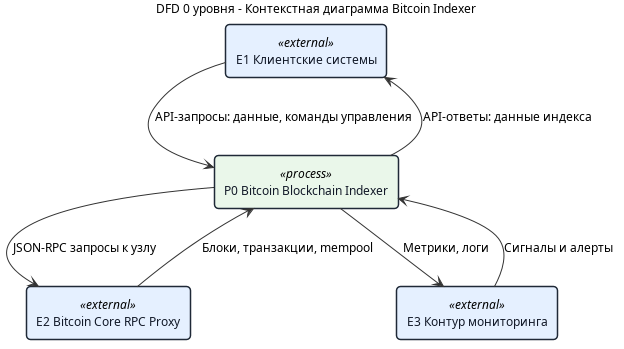
\includegraphics[width=0.9\linewidth]{../report/dfd/DFD_Level_0_Context.png}
  \caption{Контекстная DFD-диаграмма системы индексации блокчейн данных}
  \label{fig:context-dfd}
\end{figure}

Контекстная диаграмма фиксирует внешнюю границу ответственности системы. Узел
Bitcoin Core рассматривается как источник первичных блокчейн данных, PostgreSQL
--- как внешнее состояние stateless-приложения, а административной панели, CLI
и внешним клиентам доступ к индексатору предоставляется только через прикладные
интерфейсы. Такое разбиение соответствует выбранному архитектурному подходу:
серверное приложение не хранит критическое состояние локально и может быть
повторно запущено без потери прогресса индексации.

Декомпозиция контекстного процесса представлена на рисунке~\ref{fig:dfd-level-1}.
На данном уровне система разделяется на три функциональных процесса:
индексацию данных, администрирование заданий и получение/выдачу данных.
Операционное хранилище индексера отделено от хранилища конфигурации и
состояния jobs, поскольку для этих групп данных характерны разные роли в
жизненном цикле системы: первая группа отражает индексированные
блокчейн-сущности, а вторая фиксирует управляющее состояние обработки.

\begin{figure}
  \centering
  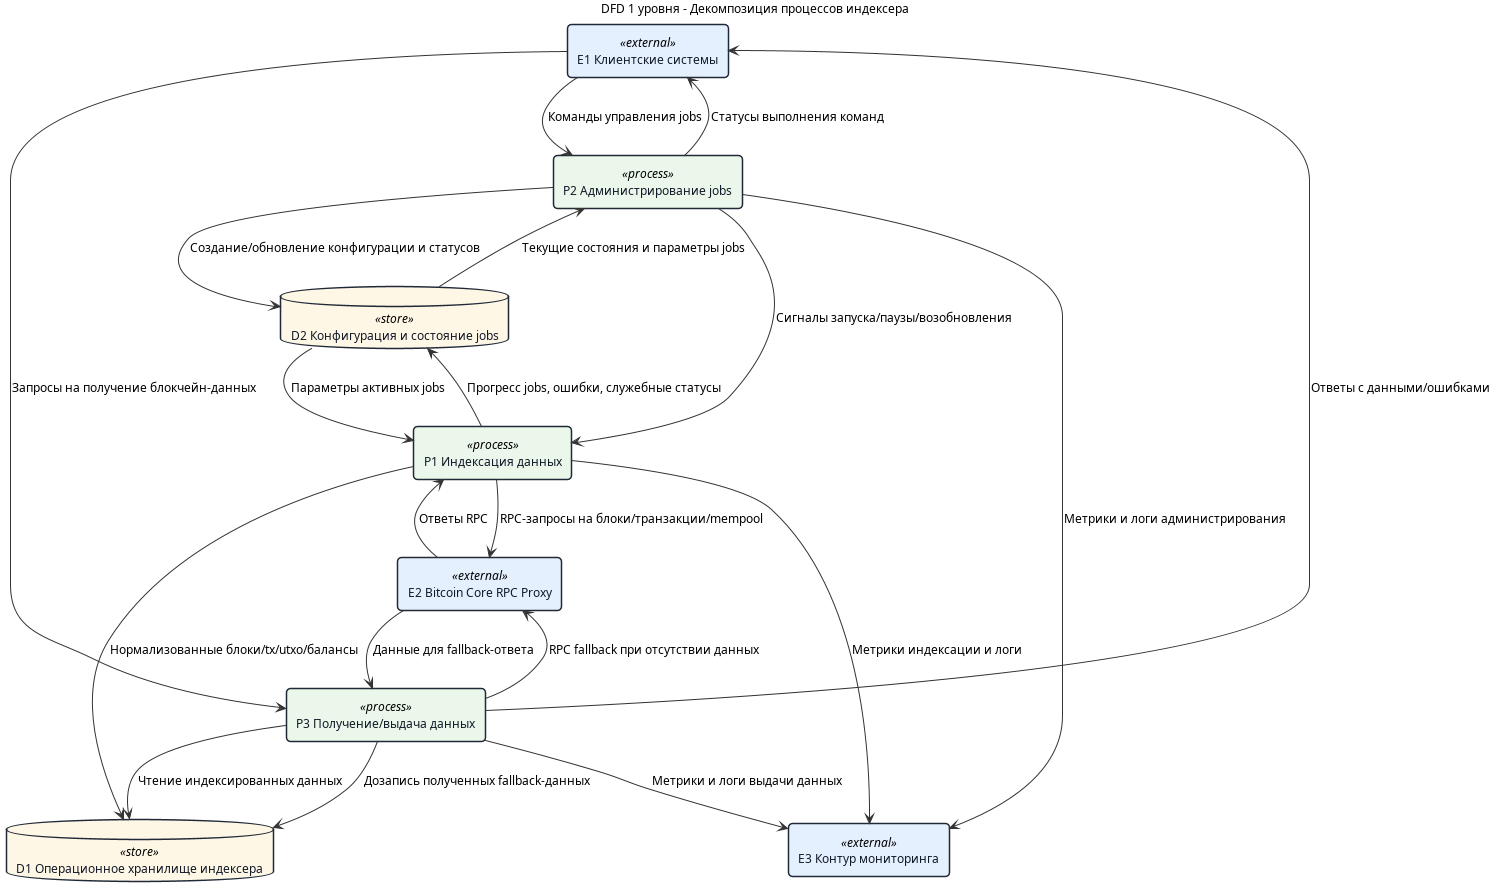
\includegraphics[width=\linewidth,height=0.72\textheight,keepaspectratio]{../report/dfd/DFD_Level_1.png}
  \caption{DFD-диаграмма первого уровня: декомпозиция процессов индексера}
  \label{fig:dfd-level-1}
\end{figure}

На диаграмме первого уровня показано, что между процессом администрирования
jobs и процессом индексации передаются только управляющие сигналы, тогда как
запись нормализованных блоков, транзакций, UTXO и балансов выполняется через
операционное хранилище. Подготовленные представления считываются из индекса, а
при необходимости допускается обращение к RPC proxy как к резервному источнику.
Такое разделение снижает связанность между контуром
управления, контуром фоновой обработки и контуром пользовательских запросов.

Критический поток подтвержденной индексации детализирован на
рисунке~\ref{fig:dfd-level-2-indexing}. Он начинается с определения tip цепи и
диапазона синхронизации, после чего выполняется загрузка блоков и транзакций,
проверка reorg, нормализация данных и фиксация прогресса задания.

\begin{figure}
  \centering
  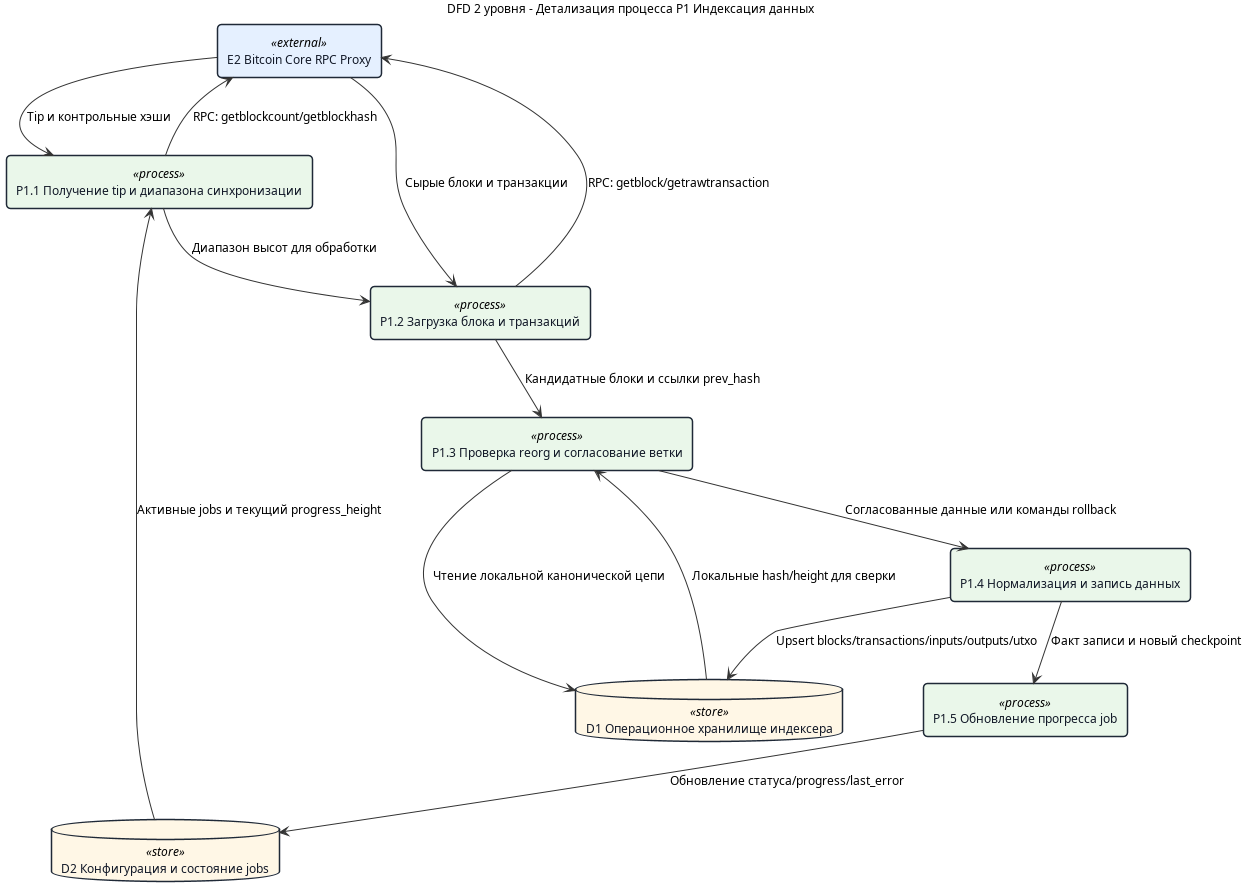
\includegraphics[width=\linewidth,height=0.72\textheight,keepaspectratio]{../report/dfd/DFD_Level_2_Indexing.png}
  \caption{DFD-диаграмма второго уровня: детализация процесса индексации данных}
  \label{fig:dfd-level-2-indexing}
\end{figure}

Декомпозиция индексации подчеркивает, что проверка согласованности цепи
выделяется в самостоятельный процесс между загрузкой блока и записью данных.
Это важно для предметной области Bitcoin: новый блок не может быть
рассмотрен изолированно, так как его связь с предыдущим хэшем определяет
принадлежность к канонической ветке. Поэтому запись в PostgreSQL выполняется
после сверки локального состояния и только затем обновляется прогресс job.

Контур управления заданиями индексирования представлен на
рисунке~\ref{fig:dfd-level-2-admin}. Он описывает обработку команд
создания, запуска, приостановки, возобновления и остановки job.

\begin{figure}
  \centering
  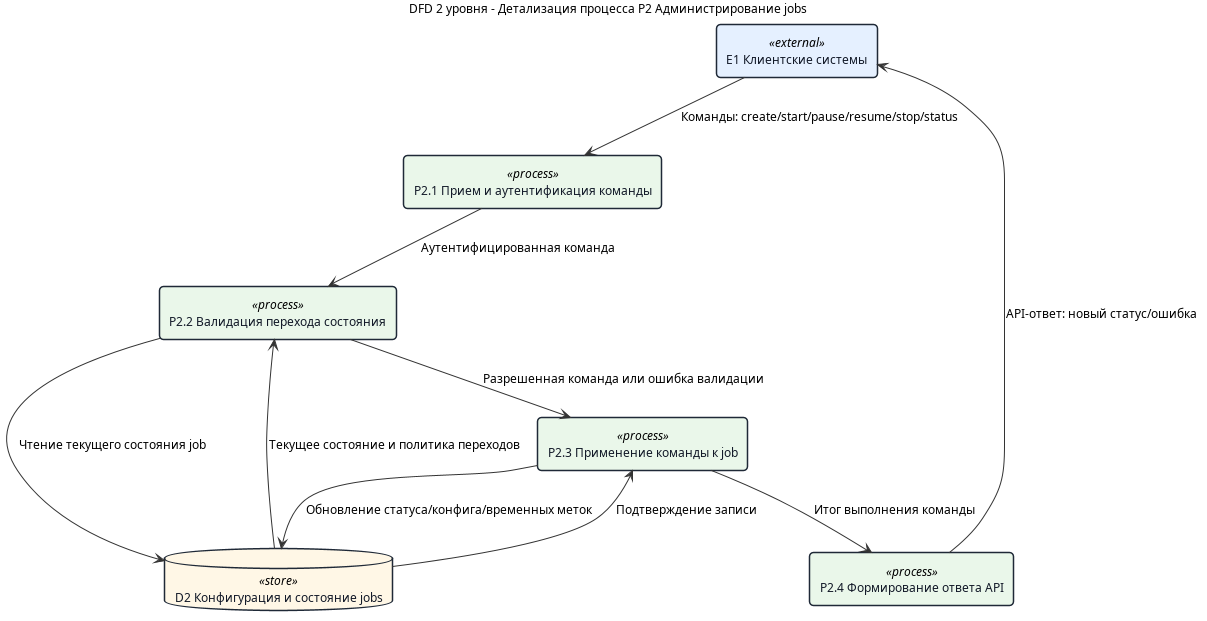
\includegraphics[width=\linewidth,height=0.68\textheight,keepaspectratio]{../report/dfd/DFD_Level_2_Admin.png}
  \caption{DFD-диаграмма второго уровня: детализация процесса администрирования jobs}
  \label{fig:dfd-level-2-admin}
\end{figure}

На этом уровне явно фиксируется, что изменение состояния задания не выполняется
непосредственно после получения команды. Сначала команда проходит
аутентификацию и валидацию допустимого перехода состояния, затем применяется к
записи job и только после этого преобразуется в API-ответ. Такое описание
обосновывает необходимость формализованного жизненного цикла задания и
согласуется с последующим описанием модуля \texttt{jobs}.

Процесс получения и выдачи данных раскрыт на
рисунке~\ref{fig:dfd-level-2-data-serving}. Диаграмма показывает обработку
прикладных запросов к блокам, транзакциям, адресам и mempool.

\begin{figure}
  \centering
  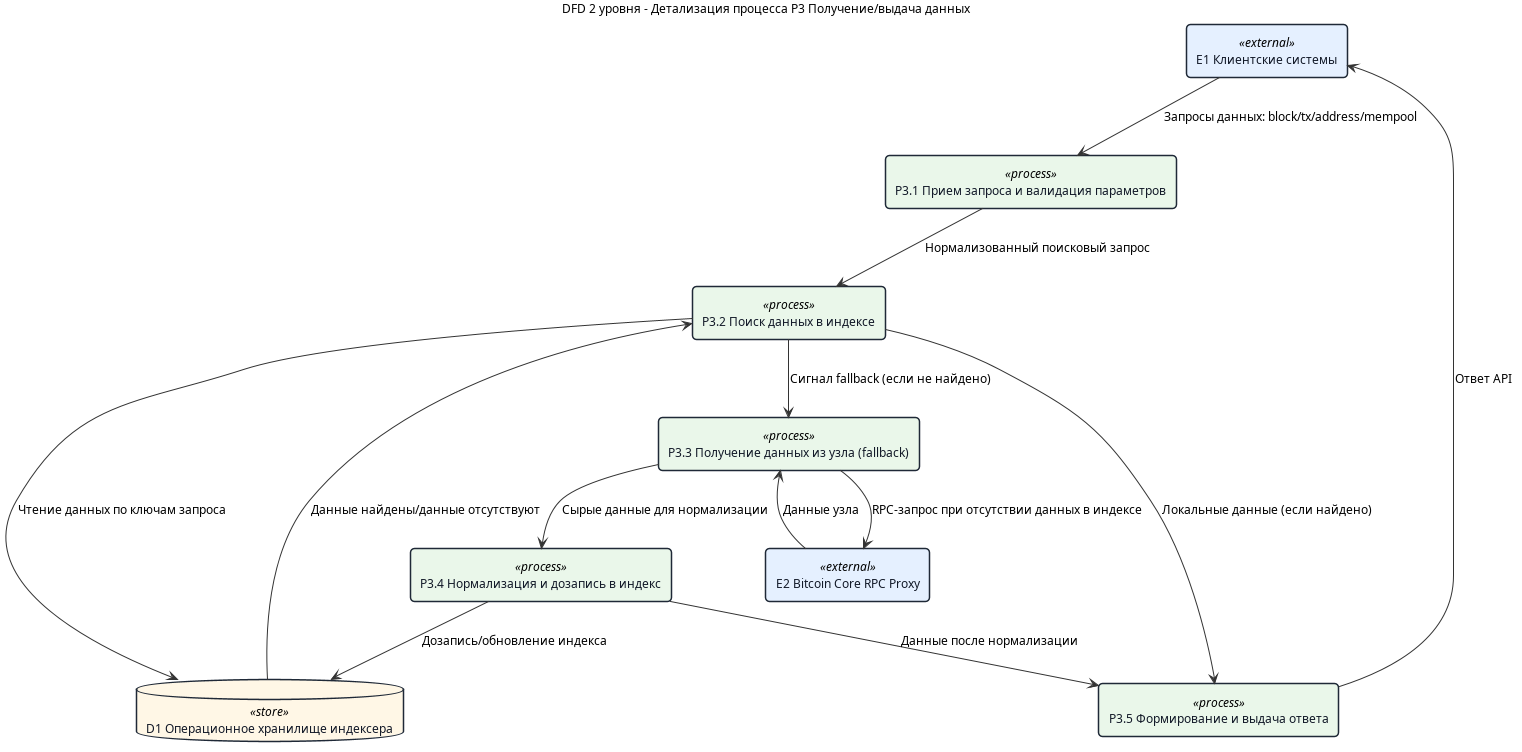
\includegraphics[width=\linewidth,height=0.72\textheight,keepaspectratio]{../report/dfd/DFD_Level_2_DataServing.png}
  \caption{DFD-диаграмма второго уровня: детализация процесса получения и выдачи данных}
  \label{fig:dfd-level-2-data-serving}
\end{figure}

Для контура выдачи данных принципиально важно разделение поиска в локальном
индексе и резервного обращения к узлу. При наличии данных ответ формируется на
основе подготовленных представлений PostgreSQL. Если данных в индексе нет,
допускается обращение к Bitcoin Core RPC proxy с последующей нормализацией и
дозаписью результата. В результате для внешнего клиента сохраняется единый API-контракт,
а внутренняя система сохраняет возможность постепенно пополнять индекс без
нарушения границ stateless backend-приложения.

С учетом особенностей предметной области итоговая постановка задачи сводится
к созданию программной системы Bitcoin Blockchain Indexer,
обеспечивающей устойчивую, управляемую и воспроизводимую индексацию
блокчейн данных сети Bitcoin, достаточную для использования в прикладных,
аналитических и исследовательских сервисах. Тем самым в работе решается
задача построения промежуточного инфраструктурного слоя между узлом Bitcoin и
внешними потребителями данных.

    \section{ПРОЕКТИРОВАНИЕ СИСТЕМЫ ИНДЕКСАЦИИ ОНЧЕЙН-ДАННЫХ}

После анализа предметной области следующим этапом является проектирование
системы, обеспечивающей устойчивую индексацию, хранение и предоставление
ончейн-данных. На данном этапе необходимо формализовать требования,
определить архитектурный подход, спроектировать состав программных модулей,
модель хранения данных и интерфейсы взаимодействия с внешними потребителями.

Проектирование системы Bitcoin Blockchain Indexer выполнялось с учетом
ограничений предметной области и требований к эксплуатационной надежности.
В качестве исходных принципов использовались модульность, управляемость
жизненного цикла заданий индексирования, транзакционная согласованность
данных и пригодность к контейнерному развертыванию
\cite{gost_arch, gost_quality, kleppmann2017designing, richards2020fundamentals, postgres_docs}. Тем самым проектирование
рассматривается не как произвольный выбор реализации, а как процесс
обоснования архитектурных решений в соответствии с выявленными требованиями.

    \subsection{Формирование функциональных и нефункциональных требований}

Требования к проектируемой системе определяются сценариями использования
ончейн-данных прикладными сервисами и особенностями самой предметной области.
В частности, система должна обеспечивать получение данных от доверенного
источника, воспроизводимую обработку подтвержденной цепи, корректную работу с
неподтвержденными транзакциями, устойчивость к reorg и удобное предоставление
результатов обработки внешним системам.

Для дальнейшего проектирования требования целесообразно разделить на
функциональные, требования к согласованности данных, эксплуатационные,
требования к безопасности и требования к расширяемости. Такая классификация
позволяет не только описать ожидаемые возможности системы, но и зафиксировать
критерии, которым должны удовлетворять архитектурные и программные решения.

\begin{table}
    \caption{Основные группы требований к системе}
    \begin{tabular}{|p{0.34\textwidth}|p{0.54\textwidth}|}\hline
    Группа требований & Содержание \\ \hline
    Функциональные & Индексация блоков, транзакций, входов, выходов, UTXO, адресных балансов, mempool-данных, управление заданиями индексирования, выдача данных через API \\ \hline
    Требования к согласованности & Идемпотентность записи, транзакционность операций, корректная обработка reorg, детерминированное обновление производных агрегатов \\ \hline
    Эксплуатационные & Контейнерное развертывание, логирование, публикация метрик, восстановление после перезапуска без потери критического состояния \\ \hline
    Требования к безопасности & Аутентификация административных операций, защищенное подключение к RPC, управление секретами через внешнюю конфигурацию и переменные окружения \\ \hline
    Требования к расширяемости & Возможность добавления новых модулей и развития системы без нарушения базовых контрактов взаимодействия \\ \hline
    \end{tabular}
    \label{tab:requirements-groups}
\end{table}

Функциональные и нефункциональные требования образуют основу всех дальнейших
проектных решений. В частности, требование stateless-характера исполнения ведет к
вынесению критического состояния в PostgreSQL, а требование воспроизводимого
развертывания обосновывает использование Docker и Docker Compose
\cite{docker_docs, compose_docs}. Требования к прикладной выдаче данных
обусловливают необходимость построения специализированной модели хранения,
ориентированной не только на запись блокчейн-событий, но и на быстрые выборки
по адресам, транзакциям, блокам и заданиям индексирования.

    \subsection{Выбор архитектурного подхода и проектирование структуры модулей}

В качестве архитектурного стандарта для разрабатываемой системы выбран
модульный монолит со stateless-характером исполнения. Данный подход позволяет
сохранить целостность приложения и упростить сопровождение системы, при этом
разделив прикладную логику на изолированные функциональные блоки с явными
границами ответственности.

Выбор именно такого архитектурного решения обусловлен следующими факторами:
\begin{enumerate}
    \item тесная связанность процессов индексации, хранения и выдачи данных;
    \item необходимость общей транзакционной модели работы с хранилищем;
    \item сравнительно ограниченный масштаб проекта по сравнению с распределенной
    микросервисной архитектурой;
    \item требование к сохранению stateless-характера приложения при хранении
    критического состояния во внешней базе данных;
    \item потребность в дальнейшем расширении за счет модулей, а не за счет
    немедленного дробления на независимые сервисы.
\end{enumerate}

С инженерной точки зрения модульный монолит в рассматриваемой задаче
представляет компромисс между целостностью доменной логики и требованием к
локализации ответственности внутри приложения. Критическое состояние при этом
хранится во внешней базе данных, что обеспечивает воспроизводимость запуска и
возможность повторного развертывания экземпляра без сохранения локального
сессионного состояния.

Компонентная структура проектируемой системы приведена на
рисунке~\ref{fig:component-c4-design}. Диаграмма отражает взаимодействие
основных модулей серверной части с внешними системами и прикладными клиентами.

\begin{figure}
  \centering
  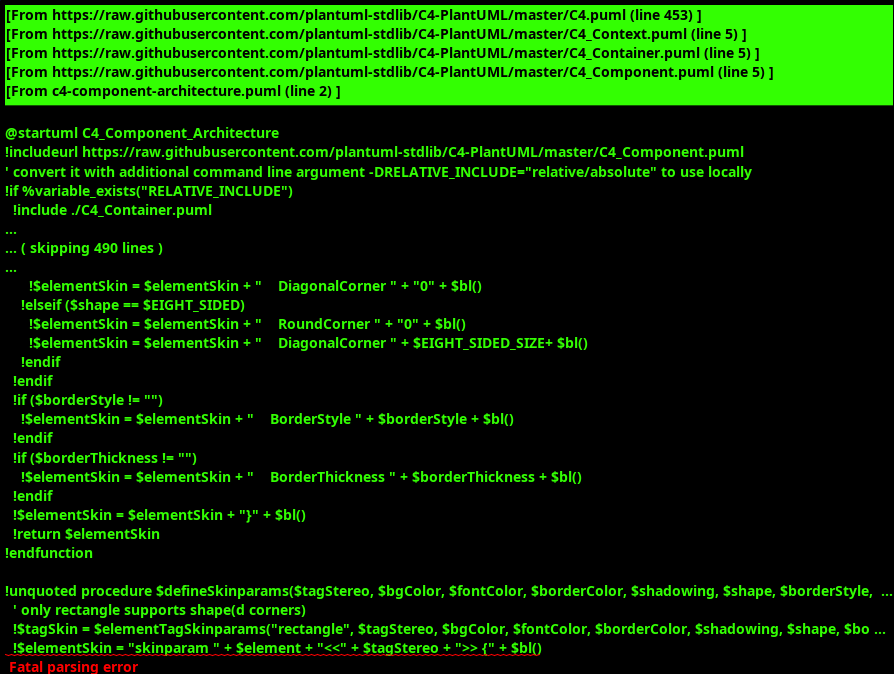
\includegraphics[width=0.9\linewidth]{../report/c4/C4_Component_Architecture.png}
  \caption{Компонентная архитектура системы индексации ончейн-данных}
  \label{fig:component-c4-design}
\end{figure}

В проектируемой системе выделены следующие основные модули:
\begin{itemize}
    \item \texttt{config} --- загрузка и валидация конфигурации, разрешение секретов;
    \item \texttt{api} --- предоставление HTTP API и маршрутизация запросов;
    \item \texttt{indexer} --- получение и сохранение подтвержденных блоков и транзакций;
    \item \texttt{jobs} --- управление заданиями индексирования и их жизненным циклом;
    \item \texttt{mempool} --- синхронизация неподтвержденных транзакций;
    \item \texttt{data} --- прикладные выборки из хранилища;
    \item \texttt{nodes} --- мониторинг состояния подключенных узлов;
    \item \texttt{storage} --- репозитории и транзакционная работа с PostgreSQL.
\end{itemize}

Такое разбиение позволяет локализовать ответственность каждого модуля,
обеспечить независимое развитие отдельных частей системы и минимизировать
влияние локальных изменений на общую архитектуру. Тем самым структура модулей
не только отражает текущую реализацию, но и служит средством обеспечения
расширяемости и сопровождаемости программного комплекса.

    \subsection{Проектирование модели данных и схемы хранения}

Для реализации функций индексирования и прикладной выдачи данных в проекте
используется реляционная модель хранения на базе PostgreSQL. Выбор данного
подхода обусловлен необходимостью обеспечения транзакционной согласованности,
поддержки ограничений целостности, эффективной индексации и формирования
многообразных выборок по связанным сущностям \cite{postgres_docs}.

Проектируемая схема хранения включает несколько классов сущностей:
\begin{enumerate}
    \item сущности первичного блокчейн-уровня: блоки, транзакции, входы и выходы;
    \item сущности текущего состояния: набор \gls{utxo}, текущие балансы адресов;
    \item сущности исторических представлений: история балансов адресов;
    \item сущности управления системой: задания индексирования и связанные с ними адресные фильтры;
    \item сущности наблюдаемости: сведения о состоянии подключенных узлов.
\end{enumerate}

В таблице~\ref{tab:data-model} представлены ключевые проектируемые таблицы,
их основные ограничения и роль в процессе индексации.

\begin{scriptsize}
\setlength{\tabcolsep}{2pt}
\begin{longtable}{|p{0.18\textwidth}|p{0.22\textwidth}|p{0.24\textwidth}|p{0.23\textwidth}|}
    \caption{Ключевые элементы модели данных}\label{tab:data-model}\\ \hline
    Таблица & Ключи и индексы & Основные поля & Роль в системе \\ \hline
    \endfirsthead
    \caption*{Продолжение таблицы \ref{tab:data-model}}\\ \hline
    Таблица & Ключи и индексы & Основные поля & Роль в системе \\ \hline
    \endhead
    \hline
    \endfoot
    \hline
    \endlastfoot
    \texttt{blocks} &
    PK \texttt{id}, unique \texttt{hash}, индексы по высоте и статусу &
    \texttt{height}, \texttt{hash}, \texttt{prev\_hash}, \texttt{status} &
    фиксация канонических и неканонических блоков \\ \hline
    \texttt{transactions} &
    PK \texttt{id}, unique \texttt{txid}, индексы по статусу, высоте и времени &
    \texttt{txid}, \texttt{block\_hash}, \texttt{block\_height}, \texttt{status} &
    связь транзакций с блоками и mempool-состояниями \\ \hline
    \texttt{tx\_outputs} &
    PK \texttt{(txid, vout)}, индекс по адресу &
    \texttt{txid}, \texttt{vout}, \texttt{address}, \texttt{value\_sats} &
    база для адресных выборок и расчета UTXO \\ \hline
    \texttt{tx\_inputs} &
    PK \texttt{(txid, vin)}, индекс по расходуемому выходу &
    \texttt{txid}, \texttt{vin}, \texttt{prev\_txid}, \texttt{prev\_vout} &
    фиксация расходования выходов \\ \hline
    \shortstack[l]{\texttt{utxos}\\\texttt{current}} &
    PK \texttt{(out\_txid, out\_vout)}, индекс по адресу и статусу &
    \texttt{address}, \texttt{value\_sats}, \texttt{status} &
    актуальное состояние непотраченных выходов \\ \hline
    \shortstack[l]{\texttt{address}\\\texttt{balance}\\\texttt{current}} &
    PK \texttt{address} &
    \texttt{confirmed\_sats}, \texttt{updated\_height} &
    быстрый ответ по текущему балансу адреса \\ \hline
    \shortstack[l]{\texttt{address}\\\texttt{balance}\\\texttt{history}} &
    PK \texttt{(address, block\_height)}, индекс по адресу и времени &
    \texttt{balance\_sats}, \texttt{block\_height}, \texttt{block\_time} &
    история изменения адресного баланса \\ \hline
    \texttt{jobs} &
    PK \texttt{job\_id}, CHECK по статусам &
    \texttt{mode}, \texttt{status}, \texttt{from\_height}, \texttt{current\_height} &
    управление жизненным циклом индексирования \\ \hline
    \shortstack[l]{\texttt{job}\\\texttt{addresses}} &
    PK \texttt{(job\_id, address)}, FK на \texttt{jobs} &
    \texttt{job\_id}, \texttt{address} &
    адресные фильтры для выборочных заданий \\ \hline
    \texttt{node\_health} &
    PK \texttt{node\_id} &
    \texttt{last\_seen\_at}, \texttt{tip\_height}, \texttt{status} &
    наблюдение за доступностью и высотой узлов \\ \hline
\end{longtable}
\end{scriptsize}

Важным свойством модели данных является ее ориентированность на
идемпотентность и воспроизводимость обработки. Для этого в проекте
используются первичные и уникальные ключи, ограничения целостности и
детерминированные правила обновления агрегатов. С инженерной точки зрения это
позволяет описать лаг индексации как
разность между высотой tip цепи и текущим прогрессом job:

\begin{equation}
    L = H_{tip} - H_{progress},
\end{equation}

где $L$ --- лаг индексирования, $H_{tip}$ --- актуальная высота цепи,
$H_{progress}$ --- высота, до которой синхронизирован job.

Данная модель хранения обеспечивает как последовательную обработку блоков, так
и эффективное выполнение прикладных запросов к уже подготовленным данным, что
является ключевым требованием к системе индексации ончейн-данных.

    \subsection{Проектирование интерфейсов взаимодействия и сценариев работы системы}

Интерфейсы проектируемой системы строятся вокруг трех основных контуров
взаимодействия: контура получения данных от узла Bitcoin, контура
административного управления и контура прикладной выдачи данных внешним
потребителям. Такое разделение позволяет формализовать назначение каждой группы
операций и уменьшить связанность между внешними участниками системы.

Контур получения данных ориентирован на доверенное взаимодействие с Bitcoin
Core через RPC-прокси. Он предназначен исключительно для внутреннего
использования индексером и не должен быть доступен прикладным клиентам. Контур
административного управления реализуется через REST API, административную
панель и CLI. В его рамках выполняются операции запуска, остановки, паузы и
возобновления заданий индексирования, а также получение сведений о состоянии узлов и
выполняемых процессов. Контур прикладной выдачи предоставляет доступ к блокам,
транзакциям, балансам адресов, UTXO и mempool-данным.

Основные проектируемые группы REST endpoints включают:
\begin{enumerate}
    \item endpoints управления заданиями индексирования;
    \item endpoints мониторинга и диагностики узлов;
    \item endpoints получения блоков, транзакций, балансов и UTXO;
    \item сервисные endpoints наблюдаемости и документирования API.
\end{enumerate}

В таблице~\ref{tab:api-groups} приведены основные группы прикладных endpoint'ов
и их назначение.

\begin{footnotesize}
\setlength{\tabcolsep}{3pt}
\begin{longtable}{|p{0.24\textwidth}|p{0.34\textwidth}|p{0.28\textwidth}|}
    \caption{Группы REST API системы}\label{tab:api-groups}\\ \hline
    Группа & Endpoint'ы & Назначение \\ \hline
    \endfirsthead
    \caption*{Продолжение таблицы \ref{tab:api-groups}}\\ \hline
    Группа & Endpoint'ы & Назначение \\ \hline
    \endhead
    \hline
    \endfoot
    \hline
    \endlastfoot
    Jobs API &
    \texttt{/v1/jobs}, \texttt{/v1/jobs/\{id\}}, операции \texttt{start}, \texttt{stop}, \texttt{pause}, \texttt{resume}, \texttt{retry} &
    создание, просмотр и управление заданиями индексирования \\ \hline
    Nodes API &
    \texttt{/v1/nodes}, \texttt{/v1/nodes/\{id\}} &
    получение сведений о подключенных узлах и их состоянии \\ \hline
    Data API &
    \texttt{/v1/data/addresses/*}, \texttt{/v1/data/transactions}, \texttt{/v1/data/blocks} &
    прикладная выдача балансов, UTXO, транзакций и блоков \\ \hline
    Observability &
    \texttt{/metrics}, OpenAPI-документация &
    мониторинг и машинно-читаемое описание контрактов API \\ \hline
\end{longtable}
\end{footnotesize}

Жизненный цикл задания индексирования формализуется набором допустимых
переходов, приведенных в таблице~\ref{tab:job-lifecycle}. Такая фиксация важна
для единообразного поведения REST API, CLI и административной панели.

\begin{footnotesize}
\setlength{\tabcolsep}{3pt}
\begin{longtable}{|p{0.17\textwidth}|p{0.27\textwidth}|p{0.22\textwidth}|p{0.22\textwidth}|}
    \caption{Допустимые переходы состояний job}\label{tab:job-lifecycle}\\ \hline
    Операция & Переход & Условие & Результат \\ \hline
    \endfirsthead
    \caption*{Продолжение таблицы \ref{tab:job-lifecycle}}\\ \hline
    Операция & Переход & Условие & Результат \\ \hline
    \endhead
    \hline
    \endfoot
    \hline
    \endlastfoot
    \texttt{start} & \texttt{created -> running} & job создан и разрешен к запуску & runner начинает обработку высот \\ \hline
    \texttt{pause} & \texttt{running -> paused} & job находится в работе & прогресс сохраняется, обработка приостанавливается \\ \hline
    \texttt{resume} & \texttt{paused -> running} & job был поставлен на паузу & обработка продолжается с сохраненной высоты \\ \hline
    \texttt{stop} & \shortstack[l]{\texttt{running|paused|}\\\texttt{failed -> created}} & требуется сброс активного выполнения & job возвращается в исходное состояние \\ \hline
    \texttt{retry} & \texttt{failed -> running} & ошибка устранена оператором & job запускается повторно с сохраненным прогрессом \\ \hline
\end{longtable}
\end{footnotesize}

Проектирование интерфейсов опирается на единый набор принципов:
\begin{enumerate}
    \item предоставление данных в прикладной форме, а не в сыром RPC-представлении;
    \item детерминированные форматы ответов и ошибок;
    \item разграничение подтвержденных данных и mempool-представлений;
    \item защита административных функций средствами аутентификации;
    \item пригодность интерфейсов для использования как человеком, так и внешними системами.
\end{enumerate}

Сценарии функционирования системы включают последовательную индексацию цепи,
обновление адресных агрегатов, обслуживание пользовательских запросов и
административное управление ходом обработки. Тем самым интерфейсы
проектируются не как набор разрозненных конечных точек доступа, а как
формализованное средство реализации основных процессов системы. В дальнейшем
именно эти сценарии становятся основой для реализации программных модулей и
для построения программы испытаний разработанного программного средства.

    \section{РАЗРАБОТКА СИСТЕМЫ ИНДЕКСАЦИИ БЛОКЧЕЙН ДАННЫХ}

\subsection{Реализация серверной части системы}

Практическая реализация проектируемой системы выполнена в виде серверного
приложения на языке Rust. Серверная часть объединяет загрузку конфигурации,
инициализацию подключений к базе данных и RPC-источнику, запуск HTTP API,
фоновых процессов обработки и средств наблюдаемости. Такой способ
организации соответствует выбранной архитектуре модульного монолита со
stateless-характером исполнения и обеспечивает единый жизненный цикл всех
компонентов приложения.

Исходный код программной реализации размещен в открытом репозитории
Bitcoin Blockchain Indexer \cite{project_github}. Репозиторий используется как
основной артефакт фиксации реализации backend-приложения, миграций,
конфигурационных файлов, вспомогательных средств запуска и материалов,
связанных с проектированием системы.

Ключевая роль серверной части заключается в координации нескольких
взаимосвязанных процессов:
\begin{enumerate}
    \item приема и валидации конфигурации запуска;
    \item синхронизации заданий индексирования из YAML-конфигурации и управляющего API;
    \item выполнения индексации подтвержденных блоков и транзакций;
    \item отдельной синхронизации состояния mempool;
    \item публикации API, метрик и диагностической информации.
\end{enumerate}

С инженерной точки зрения такое построение позволяет рассматривать систему как
единый прикладной контур обработки данных, в котором критическое состояние
сохраняется во внешней базе данных, а экземпляр приложения может быть
перезапущен без потери консистентности. Тем самым реализация серверной части
непосредственно поддерживает сформулированные ранее требования к
восстанавливаемости и управляемости системы.

Ключевые инженерные решения, использованные при реализации серверной части,
приведены в таблице~\ref{tab:implementation-decisions}. В ней архитектурные
требования соотносятся с конкретными механизмами кода и базы данных.

\begin{footnotesize}
\setlength{\tabcolsep}{3pt}
\begin{longtable}{|p{0.23\textwidth}|p{0.27\textwidth}|p{0.23\textwidth}|p{0.15\textwidth}|}
    \caption{Ключевые инженерные решения реализации}\label{tab:implementation-decisions}\\ \hline
    Решение & Назначение & Реализация & Проверка \\ \hline
    \endfirsthead
    \caption*{Продолжение таблицы \ref{tab:implementation-decisions}}\\ \hline
    Решение & Назначение & Реализация & Проверка \\ \hline
    \endhead
    \hline
    \endfoot
    \hline
    \endlastfoot
    Advisory lock на состояние цепи &
    исключить параллельную запись конфликтующих высот &
    advisory lock PostgreSQL в транзакции записи блока &
    pipeline-тесты \\ \hline
    Идемпотентная запись &
    безопасно повторять обработку блока или job &
    \texttt{ON CONFLICT}, первичные и уникальные ключи &
    storage-тесты \\ \hline
    Разделение статусов транзакций &
    не смешивать confirmed, mempool, dropped и orphaned данные &
    поле \texttt{status} и отдельные API-фильтры &
    data API тесты \\ \hline
    Пересборка агрегатов после reorg &
    восстановить UTXO и балансы по канонической ветке &
    пометка orphaned и replay canonical blocks &
    reorg-тесты \\ \hline
    Прогресс jobs в БД &
    сохранить управляемость после рестарта приложения &
    поле \texttt{progress\_height} и переходы job &
    jobs API тесты \\ \hline
    Метрики Prometheus &
    наблюдать лаг, ошибки и объем обработки &
    \texttt{/metrics}, счетчики и gauge-показатели &
    smoke-проверка \\ \hline
\end{longtable}
\end{footnotesize}

\subsection{Реализация механизма индексации блоков и транзакций}

Основной процесс обработки подтвержденных данных реализован в модуле
индексатора.
Он получает данные о блоках от Bitcoin Core, выполняет декомпозицию транзакций,
входов и выходов, после чего сохраняет результат в PostgreSQL в рамках одной
транзакции. Такой подход обеспечивает атомарность записи и предотвращает
частичное появление несогласованных данных.

Алгоритм пакетной индексации подтвержденных данных представлен на
рисунке~\ref{alg:index-batch}. В нем отражены ключевые стадии: определение
диапазона высот, проверка расхождения цепи, последовательная запись блоков и
обновление прогресса задания индексирования.

\begin{figure}
\begin{minipage}{\linewidth}
\begin{algorithm}[H]
    \SetAlgoVlined
    \KwData{конфигурация job, состояние БД, RPC-клиент}
    \KwResult{обновленные данные подтвержденной цепи и прогресс задания}
    получить текущую высоту узла\;
    определить диапазон высот для следующего батча\;
    проверить расхождение цепи в окне \texttt{reorg\_depth}\;
    \If{обнаружен reorg}{
        пометить неканонические блоки и транзакции\;
        пересобрать агрегаты UTXO и балансов\;
        откатить \texttt{progress\_height}\;
    }
    \ForEach{высота в выбранном диапазоне}{
        получить блок по RPC\;
        декомпозировать транзакции, входы и выходы\;
        сохранить блок и связанные сущности в одной транзакции БД\;
        обновить UTXO и баланс адресов\;
        обновить \texttt{progress\_height}\;
    }
\end{algorithm}
\end{minipage}
\caption{Алгоритм пакетной индексации данных подтвержденной цепи}
\label{alg:index-batch}
\end{figure}

Особое внимание в реализации уделено идемпотентности. Повторная обработка уже
сохраненной высоты не должна приводить к появлению дубликатов или искажению
адресных агрегатов. Для этого используются ограничения целостности базы
данных, транзакционная запись и согласованное обновление производных
сущностей. Таким образом, реализация индексатора обеспечивает не только
накопление данных, но и воспроизводимость результата обработки.

\subsection{Реализация управления заданиями индексирования, mempool и reorg}

Управление заданиями индексирования реализовано как отдельный функциональный
контур, обеспечивающий хранение конфигурации заданий, контроль их состояния и периодический запуск
батчей индексации. Каждое задание имеет собственный идентификатор, режим
работы, текущий статус, информацию о прогрессе и диагностические данные о
последней ошибке. Это позволяет использовать задание как единицу управляемости и
наблюдаемости процесса индексации.

Наряду с обработкой подтвержденной цепи в системе реализован отдельный контур
синхронизации mempool. Его задача состоит в периодическом опросе узла,
сохранении неподтвержденных транзакций и пометке исчезнувших записей как
\texttt{dropped}. При этом агрегаты подтвержденной цепи не смешиваются с mempool,
поскольку их семантика принципиально различается.

Алгоритм синхронизации mempool представлен на
рисунке~\ref{alg:mempool-sync}.

\begin{figure}
\begin{minipage}{\linewidth}
\begin{algorithm}[H]
    \SetAlgoVlined
    \KwData{список известных mempool tx, ответ \texttt{getrawmempool}}
    \KwResult{актуальное состояние mempool в БД}
    получить текущий список \texttt{txid} из mempool\;
    определить новые и исчезнувшие транзакции\;
    \ForEach{новый \texttt{txid}}{
        запросить verbose-представление транзакции\;
        сохранить запись со статусом \texttt{mempool}\;
        сохранить входы и выходы для будущей фильтрации по адресу\;
    }
    \ForEach{исчезнувший \texttt{txid}}{
        пометить запись как \texttt{dropped}, если она не подтверждена\;
    }
\end{algorithm}
\end{minipage}
\caption{Алгоритм синхронизации mempool}
\label{alg:mempool-sync}
\end{figure}

Для обеспечения корректности данных канонической цепи в системе реализована обработка
reorg. При обнаружении расхождения между сохраненной в БД цепью и актуальным
состоянием узла неканонические блоки переводятся в статус \texttt{orphaned},
затронутым транзакциям присваивается соответствующая маркировка, а производные
агрегаты пересобираются по оставшейся канонической ветке. Одновременно
прогресс задания индексирования откатывается до согласованной высоты, после чего индексация
продолжается уже по новой ветви цепи.

\subsection{Реализация API, конфигурирования и мониторинга}

Внешнее взаимодействие с системой реализовано через REST API, которое
предоставляет операции управления заданиями индексирования, диагностики узлов и получения
проиндексированных данных. Для сопровождения системы предусмотрены также
административная панель и CLI, работающие поверх того же HTTP-контракта.

Конфигурирование серверного приложения выполняется через YAML-файл и переменные окружения.
В конфигурации задаются параметры API, настройки подключения к RPC-узлу,
ограничения параллелизма, параметры заданий индексирования и режимы обработки mempool и reorg.
Такой подход делает конфигурацию внешней по отношению к приложению и хорошо
согласуется с требованиями контейнерного развертывания.

Наблюдаемость системы обеспечивается за счет JSON-логирования и публикации
метрик Prometheus. В частности, экспортируются показатели текущей высоты цепи,
прогресса заданий индексирования, лага индексации, числа обработанных блоков и транзакций,
латентности RPC-вызовов и ошибок ключевых подсистем. Это позволяет использовать
разработанную систему как основу для реального эксплуатационного контура и
подтверждает соответствие реализованных средств сопровождения исходным
эксплуатационным требованиям.

    \subsection{Кодовые фрагменты, иллюстрирующие реализацию}

Для подтверждения того, что изложенные проектные решения реализованы в кодовой
базе, в работе приведены листинги ключевых фрагментов программной системы.
Они выбраны не по признаку краткости, а по связи с критическими требованиями:
транзакционная согласованность, идемпотентность обработки и управляемость
жизненного цикла заданий индексирования.

На рисунке~\ref{src:src1} приведен фрагмент метода сохранения блока. Он
показывает начало транзакционной записи, использование advisory lock для
синхронизации состояния цепи, проверку повторной обработки уже сохраненной
высоты и ожидание предыдущего блока перед записью следующей высоты. Данный
фрагмент непосредственно связан с требованиями корректной обработки
подтвержденной цепи, идемпотентности и устойчивости к повторному запуску job.

\begin{figure}
\lstinputlisting[firstline=77,lastline=96]{../src/modules/indexer/mod.rs}
\caption{Фрагмент транзакционной и идемпотентной записи блока}
\label{src:src1}
\end{figure}

На рисунке~\ref{src:src2} приведена функция, задающая допустимые переходы
состояний job. Именно этот фрагмент делает жизненный цикл задания
формализованным контрактом: недопустимые переходы возвращают ошибку, а REST API,
CLI и административная панель используют единую бизнес-логику управления
индексированием.

\begin{figure}
\lstinputlisting[firstline=575,lastline=585]{../src/modules/jobs/mod.rs}
\caption{Фрагмент проверки допустимых переходов job}
\label{src:src2}
\end{figure}

Командный интерфейс реализован в отдельном модуле \texttt{cli/indexer\_cli.py}
и используется для вспомогательного взаимодействия с заданиями индексирования,
узлами и прикладными данными через тот же REST API, что и административная
панель.

    
    \section{ИССЛЕДОВАНИЕ И ОЦЕНКА КАЧЕСТВА РАЗРАБОТАННОЙ СИСТЕМЫ}

\subsection{Цели и задачи испытаний}

После реализации программной системы необходима проверка того, что полученное
решение соответствует сформулированным требованиям и сохраняет корректность
работы в ключевых для предметной области сценариях. Для системы индексации
ончейн-данных такая проверка должна охватывать не только общие API-функции, но
и устойчивость к reorg, корректность работы с mempool, согласованность
хранилища и работоспособность управляющих механизмов.

Целью испытаний является подтверждение пригодности разработанной системы
\texttt{Bitcoin Blockchain Indexer} к решению задач индексации, хранения и
выдачи ончейн-данных. Для достижения этой цели
необходимо решить следующие задачи:
\begin{enumerate}
    \item проверить корректность функций управления заданиями индексирования и взаимодействия с API;
    \item проверить согласованность записи подтвержденных данных в хранилище;
    \item оценить корректность обработки mempool и реорганизаций цепи;
    \item подтвердить работоспособность механизмов мониторинга и диагностики;
    \item сопоставить фактические результаты с установленными критериями проверки.
\end{enumerate}

\subsection{Программа и методика испытаний}

Испытания системы строятся на сочетании интеграционного тестирования,
функциональной проверки API и анализа критериев приемки. В качестве
основного подхода используются тесты, запускаемые в окружении с контейнером
PostgreSQL через \texttt{testcontainers}, что позволяет приблизить условия
проверки к реальной эксплуатации, сохраняя воспроизводимость тестовых
сценариев \cite{testcontainers_docs}.

В рамках программы испытаний проверяются следующие группы сценариев:
\begin{enumerate}
    \item сценарии жизненного цикла заданий индексирования: создание, запуск, пауза,
    возобновление, остановка и обработка ошибочных переходов;
    \item сценарии API nodes и data API, включая запросы балансов, UTXO,
    транзакций, блоков и mempool-данных;
    \item сценарии работы контура индексации и проверки идемпотентности
    записи подтвержденных блоков;
    \item сценарии фоновых процессов обработки, включая синхронизацию mempool и обработку reorg;
    \item сценарии наблюдаемости, связанные с публикацией метрик и
    диагностической информации о состоянии узлов и заданий индексирования.
\end{enumerate}

Методически испытания ориентированы на подтверждение ключевых свойств системы:
функциональной корректности, согласованности данных, восстанавливаемости после
сбоев и эксплуатационной наблюдаемости. Для итоговой оценки используется
перечень критериев приемки, фиксирующий степень выполнения отдельных
требований.

\subsection{Проверка корректности функциональных возможностей}

Функциональная корректность системы подтверждается набором интеграционных
тестов и реализованными прикладными сценариями взаимодействия с API.
Проверяются операции управления заданиями индексирования, получение списка узлов, запросы
подтвержденных транзакций, балансов адресов, UTXO и блоков, а также
пограничные ситуации, связанные с ошибками авторизации, отсутствием объекта
или нарушением ограничений переходов состояний.

С точки зрения предметной области особенно важны результаты проверки следующих
свойств:
\begin{enumerate}
    \item задания индексирования обладают формализованным жизненным циклом и корректно меняют
    состояние через API;
    \item подтвержденные данные сохраняются в БД в виде связанных сущностей:
    блоков, транзакций, входов, выходов и агрегатов адресного уровня;
    \item mempool-данные доступны как отдельный класс сущностей и не смешиваются
    с представлениями подтвержденной цепи;
    \item выдача данных через API ориентирована на прикладные выборки, а не на
    сырые RPC-ответы.
\end{enumerate}

Таким образом, функциональное тестирование показывает, что разработанная
система реализует основной набор возможностей, предусмотренный
сформулированными требованиями к программному комплексу, и обеспечивает
прикладную форму доступа к данным, отличную от прямой работы с RPC узла.

\subsection{Оценка устойчивости к reorg и изменениям состояния mempool}

Для систем индексации ончейн-данных устойчивость к изменениям состояния сети
является одним из ключевых критериев качества. В рассматриваемом проекте это
свойство проверяется через сценарии, связанные с reorg и динамикой mempool.

Испытания reorg подтверждают, что при обнаружении расхождения между сохраненной
в БД цепью и актуальными данными узла система:
\begin{enumerate}
    \item помечает затронутые блоки как неканонические;
    \item переводит связанные транзакции в статус \texttt{orphaned};
    \item пересчитывает производные агрегаты по оставшейся канонической ветке;
    \item откатывает прогресс задания индексирования до согласованной высоты.
\end{enumerate}

Испытания mempool подтверждают, что фоновый процесс синхронизации корректно обрабатывает появление
новых неподтвержденных транзакций и помечает исчезнувшие как
\texttt{dropped}. При этом текущие балансы подтвержденной цепи и подтвержденные \gls{utxo}
не искажаются за счет временного состояния mempool. Такое разделение
представлений принципиально важно для достоверности прикладных ответов.

Следовательно, система демонстрирует устойчивость к двум наиболее характерным
для предметной области видам изменчивости: локальному пересмотру канонической
цепи и колебаниям состава неподтвержденных транзакций.

\subsection{Оценка эксплуатационных характеристик и наблюдаемости}

Помимо функциональной корректности, для практического использования системы
важны ее эксплуатационные свойства. В разработанном решении они обеспечиваются
через контейнеризованное развертывание, конфигурирование из внешних источников,
JSON-логирование и публикацию метрик Prometheus \cite{prometheus_docs}.

К числу значимых эксплуатационных характеристик относятся:
\begin{enumerate}
    \item воспроизводимость запуска серверного приложения и базы данных в контейнерном окружении;
    \item возможность мониторинга прогресса заданий индексирования и текущей высоты цепи;
    \item наблюдение за RPC-запросами, задержками и ошибками записи в БД;
    \item наличие диагностической информации по состоянию узлов;
    \item пригодность системы к сопровождению через API, CLI и административную панель.
\end{enumerate}

В проекте экспортируются метрики текущей высоты цепи, прогресса заданий индексирования, лага
индексации, количества обработанных блоков и транзакций, а также статистика
RPC-запросов и ошибок. Это позволяет использовать систему как основу для последующей эксплуатационной
интеграции.

\subsection{Анализ результатов испытаний}

Анализ выполненных испытаний показывает, что основная часть требований к системе
реализована и подтверждена кодом, интеграционными тестами и критериями
приемки. Наиболее полно подтверждены работоспособность схемы хранения,
жизненный цикл заданий индексирования, корректность записи подтвержденных данных, обработка reorg,
разделение mempool и подтвержденной цепи, а также наличие REST API, CLI и
административной панели.

Вместе с тем анализ результатов испытаний показывает наличие направлений,
требующих дальнейшего расширения экспериментальной проверки. К ним относятся
подтверждение защищенного эксплуатационного контура взаимодействия,
полномасштабные end-to-end испытания с реальным Bitcoin Core/regtest и более
детальная фиксация итоговых показателей покрытия серверной части тестами.
Указанные вопросы не ставят под сомнение достигнутую работоспособность
системы, однако определяют перспективы углубления ее верификации.

В целом результаты испытаний позволяют сделать вывод о том, что разработанная
система успешно решает основную задачу индексации ончейн-данных, а выбранные
архитектурные и проектные решения являются обоснованными с точки зрения
предметной области и дальнейшего развития проекта.

\section{ПРАКТИЧЕСКАЯ ЗНАЧИМОСТЬ И ПЕРСПЕКТИВЫ РАЗВИТИЯ СИСТЕМЫ}

\subsection{Практическая значимость разработанного решения}

Практическая значимость разработанной системы определяется тем, что она
формирует специализированный слой доступа к ончейн-данным Bitcoin, пригодный
для использования прикладными и аналитическими сервисами. В отличие от прямой
работы с узлом сети, такое решение предоставляет уже нормализованные и
подготовленные данные, что снижает сложность интеграции и уменьшает нагрузку
на инфраструктуру источника данных.

Для практического применения наиболее важны следующие свойства разработанной
системы:
\begin{enumerate}
    \item наличие прикладного API для доступа к блокам, транзакциям, UTXO,
    балансам адресов и состоянию заданий индексирования;
    \item возможность управляемой индексации с контролем прогресса и ошибок;
    \item наличие административных и вспомогательных средств сопровождения;
    \item готовность к контейнерному развертыванию и мониторингу;
    \item сохранение согласованности данных подтвержденной цепи при reorg и при работе с mempool.
\end{enumerate}

\subsection{Возможности применения системы в прикладных сервисах}

Разработанная система может использоваться в составе различных программных
решений, работающих с блокчейн-данными Bitcoin. В частности, она подходит для:
\begin{enumerate}
    \item аналитических сервисов, выполняющих выборки по адресам, транзакциям и блокам;
    \item административных и мониторинговых панелей, отображающих состояние узлов и заданий индексирования;
    \item внутренних корпоративных сервисов, которым требуется контролируемый
    доступ к ончейн-данным без прямого обращения к RPC узла;
    \item исследовательских и учебных стендов, демонстрирующих процессы
    индексации, хранения и предоставления блокчейн-данных.
\end{enumerate}

Наличие CLI и административной панели расширяет область практического
использования системы, поскольку позволяет применять ее как в автоматизированных
сценариях, так и в задачах оперативного сопровождения.

\subsection{Ограничения текущей версии системы}

Несмотря на достижение основной цели работы, текущая версия системы
имеет ряд ограничений. К ним относятся:
\begin{enumerate}
    \item неполное подтверждение end-to-end сценариев с реальным Bitcoin Core;
    \item необходимость дальнейшего подтверждения защищенного эксплуатационного контура взаимодействия;
    \item ограниченная глубина экспериментальной оценки производительности;
    \item применение общей стратегии индексации без специализированной
    оптимизации для отдельных пользовательских режимов, например \texttt{address\_list};
    \item отсутствие расширенного эксплуатационного alerting и более детальных
    сценариев деградации узлов.
\end{enumerate}

Указанные ограничения не снижают значимости достигнутого результата, но
определяют границы текущего этапа разработки и подтверждают, что система
находится на стадии, ориентированной на дальнейшее инженерное развитие.

\subsection{Направления дальнейшего развития системы}

Перспективы развития разработанной системы связаны как с углублением
функциональности, так и с расширением эксплуатационных возможностей. Наиболее
естественными направлениями дальнейшей работы являются:
\begin{enumerate}
    \item проведение полноценных end-to-end испытаний с реальным узлом Bitcoin Core;
    \item развитие защищенного контура взаимодействия серверной части и внешних клиентов;
    \item оптимизация производительности индексирования и прикладных выборок;
    \item расширение режимов работы заданий индексирования и стратегий фильтрации по адресам;
    \item развитие средств мониторинга, диагностики и автоматического реагирования;
    \item подготовка архитектурной базы для дальнейшего масштабирования решения.
\end{enumerate}

С учетом выбранного архитектурного подхода указанные направления могут быть
реализованы поэтапно без отказа от уже созданной модели хранения и структуры
основных модулей.

\subsection{Выводы по результатам работы}

Разработанная система индексации ончейн-данных обладает практической ценностью
как самостоятельный программный компонент, обеспечивающий контролируемое
получение, хранение и выдачу блокчейн-данных Bitcoin. Ее применение позволяет
снизить сложность интеграции прикладных сервисов с блокчейн-инфраструктурой и
создает основу для дальнейшего развития в сторону более полного промышленного
решения.

\conclusion

В выпускной квалификационной работе решена задача проектирования и разработки
системы индексации ончейн-данных сети Bitcoin. В процессе выполнения работы
были последовательно рассмотрены теоретические основы предметной области,
проанализированы особенности блокчейна Bitcoin как источника данных,
сформированы требования к системе, спроектированы архитектура программного
комплекса и модель хранения, а также описана реализация ключевых модулей
индексации, управления, мониторинга и прикладной выдачи данных.

В результате выполненной работы создан программный комплекс
\texttt{Bitcoin Blockchain Indexer}, реализующий индексацию блоков и
транзакций, поддержку текущего состояния \gls{utxo}, адресных балансов,
обработку mempool и reorg, управление заданиями индексирования, а также предоставление
данных через REST API, административную панель и CLI. Проведенные испытания
подтвердили работоспособность основных функций системы и показали обоснованность
выбранных архитектурных и проектных решений.

Практическая значимость работы состоит в создании основы для дальнейшего
развития инфраструктурного решения, предназначенного для использования в
прикладных и аналитических сервисах, работающих с ончейн-данными Bitcoin.
Полученные результаты могут быть использованы как для дальнейшей инженерной
доработки проекта, так и для развития исследований в области системной
индексации блокчейн-данных.
 % Заключение

    \printbibliography % Список литературы

    \appendix % Приложения
    \appendixsection{Диаграмма контейнерного развёртывания}

В приложении приведена схема контейнерного развёртывания проекта.
Рисунок~\ref{fig:a1} использует подготовленный в каталоге \texttt{report}
архитектурный артефакт и показывает состав runtime-окружения: backend,
PostgreSQL, административную панель, прокси-слой и внешний Bitcoin RPC узел.

\begin{figure}
    \centering
    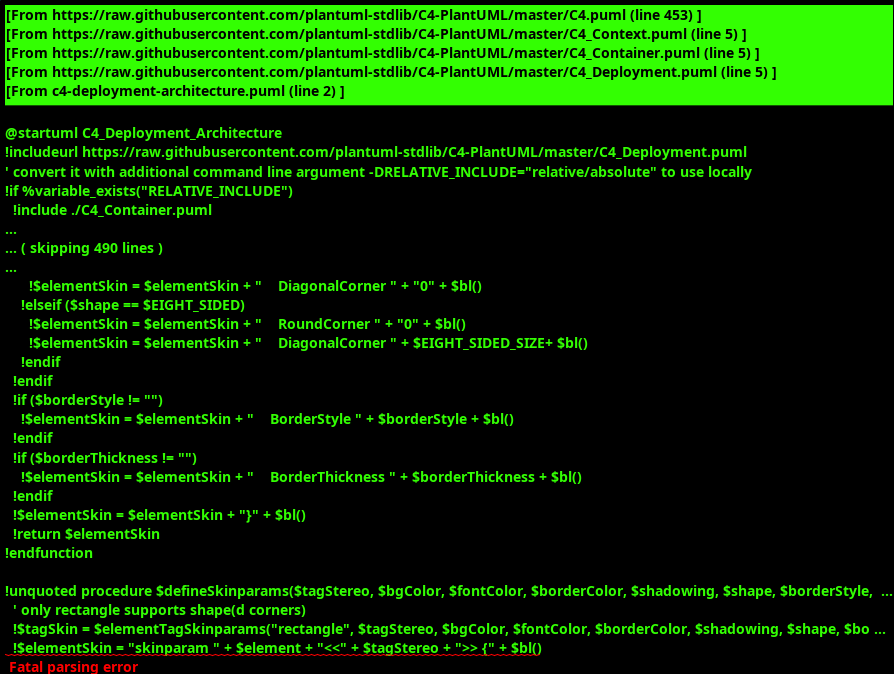
\includegraphics[width=\linewidth]{../report/c4/C4_Deployment_Architecture.png}
    \caption{Контейнерное развёртывание системы}
    \label{fig:a1}
\end{figure}

    \appendixsection{Репозиторий проекта}

Исходный код разработанной системы размещен в репозитории GitHub:
\url{https://github.com/vivichv9/Blockchain-Indexer}. Репозиторий содержит
материалы реализации, конфигурационные файлы, миграции базы данных,
административную панель и документацию проекта.

Для перехода к репозиторию также может использоваться QR-код,
представленный на рисунке~\ref{fig:github-qr}.

\begin{figure}
    \centering
    \href{https://github.com/vivichv9/Blockchain-Indexer}{%
        
\includegraphics[width=0.34\linewidth]{inc/github_qr.png}%
    }
    \caption{QR-код для перехода к репозиторию проекта}
    \label{fig:github-qr}
\end{figure}

    \appendixsection{Фрагмент конфигурации индексатора}

В приложении приведен сокращенный пример конфигурации индексатора. Полная
конфигурация хранится в файле \texttt{config/indexer.yaml}; здесь оставлены
только параметры, необходимые для понимания структуры настройки серверной
части, RPC-подключения, индексатора и задания синхронизации.

\begin{lstlisting}[
language={},
numbers=none,
basicstyle=\ttfamily\footnotesize,
caption={Сокращенный пример конфигурации системы индексации},
label={src:src3}
]
server:
  bind_host: "0.0.0.0"
  bind_port: 8080
  auth:
    basic:
      username: "admin"
      password_env: "INDEXER_API_PASSWORD"

rpc:
  node_id: "btc-testnet-1"
  url: "https://rpc.example.com"
  auth:
    basic:
      username: "rpcuser"
      password_env: "BITCOIN_RPC_PASSWORD"
  mtls:
    enabled: false

indexer:
  network: "testnet"
  reorg_depth: 12
  poll:
    tip_interval_ms: 5000
    mempool_interval_ms: 3000

jobs:
  - job_id: "full-sync"
    mode: "all_addresses"
    enabled: true
\end{lstlisting}

\end{document}
